\documentclass[11pt, oneside]{article} 
\usepackage{geometry}
\geometry{letterpaper} 
\usepackage{graphicx}
	
\usepackage{amssymb}
\usepackage{amsmath}
\usepackage{parskip}
\usepackage{color}
\usepackage{hyperref}

\graphicspath{{/Users/telliott_admin/Dropbox/Tex/png/}}
% \begin{center} 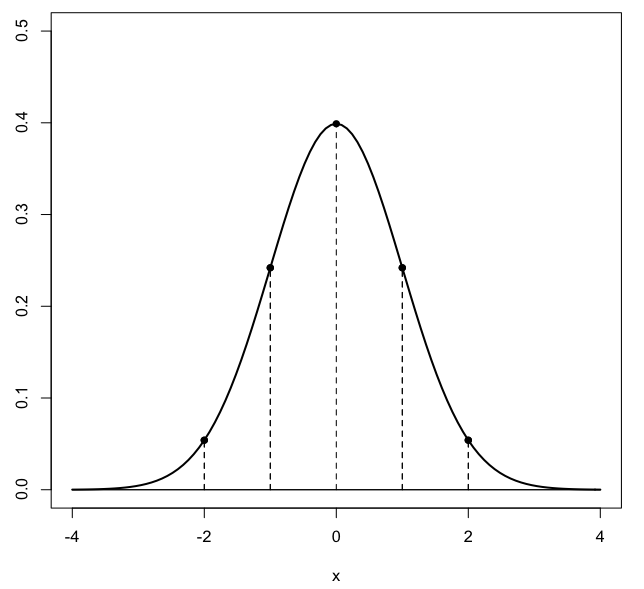
\includegraphics [scale=0.4] {gauss3.png} \end{center}

\title{Polynomial arithmetic}
\date{}

\begin{document}
\maketitle
\Large

As you know, a polynomial is an expression of the form:
\[ \sum_0^n a_n x^n \]

where the coefficients come from some set S, for example, the integers:
\[ x^5 + 9x^3 + 2x^2 + 1 \]

This is a polynomial \emph{of degree} 5.

Polynomial arithmetic deals with addition, multiplication, etc. of polynomials.

Consider this example of division for polynomials with cofactors from the set of real numbers:
\[ \frac{8x^2 + 3x + 2 }{2x + 1} \]

The first term of the quotient is $4x$ (because $4x \times 2x = 8x^2$) and 
\[ 4x \times (2x+1) = 8x^2 + 4x \]

so we subtract that from the numerator and the remainder is $-x + 2$ and dividing again
\[ \frac{-x + 2}{2x + 1} \]

The second term of the quotient is $-0.5$ (because $-0.5 \times 2 = -1$ and
\[ -0.5 \times (2x + 1) = -x - 0.5 \]
Subtracting $-0.5$ from $2$ leaves a remainder of $2.5$.

\subsection*{cofactors 0 or 1}

The polynomials that we use for cryptography have cofactors $a_n$ equal to either $0$ or $1$.  Thus

\[ 1 \cdot x^5 + 0 \cdot x^4 + 1 \cdot x^3 + 1 \cdot x^2 + 1\cdot x^1 + 1 \cdot x^0 \]

The terms with zero for the coefficient are not written, the coefficients $1$ are suppressed, as so are the exponents for $x^1$ and $x^0$, thus:

\[  x^5 + x^3 + x^2 +  x + 1 \]

There are two other representations of polynomials that we'll use quite a bit.  The first is to write the coefficients as a binary number:
\begin{verbatim}
101111 = x^5 + x^3 + x^2 + x + 1
\end{verbatim}

The other is to write a digit for the exponent, if the cofactor is not zero, with appropriate spacing:
\begin{verbatim}
5 . 3 2 1
\end{verbatim}

but without the dot
\begin{verbatim}
5   3 2 1
\end{verbatim}

\subsection*{addition and multiplication}

Polynomial addition is XOR ($\oplus$):
\[ (x^2 + x) + (x^2 + 1) = x + 1 \]

In the extended Euclidean algorithm, we will see numbers with a negative cofactor.  Since
\[ 1 + 1 = 0 = 1 - 1 \]
\[ 1 = - 1\]
All minus signs can just be dropped.  Subtraction is the same as addition.

Polynomial multiplication is as you would expect:
\[ (x^2 + x)(x^3 + x + 1) = x^5 + x^3 + x^2 + x^4 + x^2 + x \]

except that we also do XOR:
\[ = x^5 +x^4 + x^3 + x \]

Using the binary notation:
\begin{verbatim}
  01011 = x^3 + x + 1
  00110 = x^2 + x
  -----
  10110
 10110
 ------
 111010 = x^5 +x^4 + x^3 + x
\end{verbatim}

The same calculation in reverse.

\begin{verbatim}
  00110 = x^2 + x
  01011 = x^3 + x + 1
  -----
    110
   110
 110
 ------
 111010 = x^5 +x^4 + x^3 + x
\end{verbatim}

Multiplication by $x$ is the same as multiplication by binary $10$.  It is a left-shift of one place.  Multiplication by $100$ is a left-shift of two places.  Multiplication by $n$ consists of multiplication by each binary digit of $n$, followed by XOR.

The results are not the same as from decimal multiplication:  $110$ is $6$ and $1011$ is $11$, but $111010$ is \emph{not} $66$.  It is $32 + 16 + 8 + 2 = 58$.

There is an additional operation that we are not explaining yet, but don't forget it when the time comes:  division by an "irreducible polynomial".

Pseudocode for my routine to multiply $a \times b$ in Python:

\begin{verbatim}  
if a < b:
    switch a,b
reverse the digits of b
r = 0
for each digit c in b (reversed):
    if c == '1':
        r = r ^ a    # addition
    a = a << 1    # left-shift
return r
\end{verbatim}

\subsection*{Division}
In decimal, multiplication is repeated addition.  This is not true in the new system.
 
\[ 110 * 1011 = 10 * 1011 + 100 * 1011 \]
\[ \ne (1011 + 1011) + (1011 + 1011 + 1011 + 1011) \]
Instead, what we've written is just equal to zero.

Multiplication is repeated left-shift by the number of  binary digits in the multiplicand, followed by XOR.

In the same way, division is not repeated subtraction (addition).  But it has actually the same definition as multiplication.  Example:

\begin{verbatim}
111010 = x^5 +x^4 + x^3 + x
1011     = (x^3 + x + 1) * (x^2)
 ----
 10110
 1011   = (x^3 + x + 1) * (x)
 ----
 00000
\end{verbatim}

As we saw, $x^5 +x^4 + x^3 + x$ is evenly divided by $(x^3 + x + 1$.  The quotient is $x^2 + x$ (we moved over two units above, and then one unit), and the remainder is $0$.

When we do division for the fields to be constructed, division will be by an "irreducible" polynomial.  Such a polynomial has no factors in the field, and so the result will never be zero.  Justification for this statement will be coming shortly.

Recall that in the definition of a field, the crucial new component was possession of a multiplicative inverse for each element of the field.  For every $a$ there exists a $b$ such that:   $ab = 1$.

Then, we can define division by $c$ as multiplication by the inverse of $c$:
\[ \frac{a}{c} = ab, \ \ \ \ \text{if} \ \ \ \ bc = 1 \]

\end{document}